
%(BEGIN_QUESTION)
% Copyright 2010, Tony R. Kuphaldt, released under the Creative Commons Attribution License (v 1.0)
% This means you may do almost anything with this work of mine, so long as you give me proper credit

Sketch the wires necessary to connect two limit switches (normally-closed contacts) to input channels {\tt Ix.5} and {\tt Ix.11} of a Siemens SM 321 discrete input card (model 6ES7321-1BH50-0AA0).  The internal schematic diagram of the first channel ({\tt Ix.0}) is shown as ``typical'' for all the channels:

$$\includegraphics[width=15.5cm]{i02508x01.eps}$$

Also, identify whether this is a {\it sinking} or a {\it sourcing} input card, and sketch the directions of all currents through your sketched wires.

\vfil 

\underbar{file i02508}
\eject
%(END_QUESTION)





%(BEGIN_ANSWER)

This is a graded question -- no answers or hints given!

%(END_ANSWER)





%(BEGIN_NOTES)

This is an {\it input} PLC card, and so it receives electric current from a sensing device (e.g. a limit switch) to tell the PLC's microprocessor whether the sensor has been triggered or not.  Looking at the input card's internal circuitry, we see an optocoupler (LED and phototransistor) used to connect the interface circuitry with the real-world sensor signal.  In order to turn this phototransistor on, the LED must become forward-biased.

In order for the photocoupler's LED to become forward-biased, we must have direct current flowing downward through it (conventional flow notation).  This tells us the necessary direction of sensor current into the card: current enters in the L+ terminal, exiting the respective I/O channel terminal.  Since the L+ terminal is the ``common'' terminal for all 16 inputs on this particular card, it must be connected to the positive pole of a DC power supply.  Each limit switch must then be connected to the DC supply's negative pole, sinking current from the respective channels of the input card:

$$\includegraphics[width=15.5cm]{i02508x02.eps}$$

This particular input card is the {\it sourcing} type (arrows drawn in the direction of conventional flow).

%INDEX% PLC, I/O: discrete I/O device wiring

%(END_NOTES)


